\chapter{Evaluation}
\label{chap:evaluation}

In this chapter, we first define the goals of our evaluation in \autoref{sec:goals}. Subsequently, we describe the methodology to achieve these goals in \autoref{sec:methodology}, followed by the experimental setup in \autoref{sec:setup}. Finally, we present the benchmarks in \autoref{sec:benchmarks} and discuss the results in \autoref{sec:discussion}.

\section{Goals}
\label{sec:goals}
%
Referring back to our research objectives from \autoref{sec:research-objectives}, the goals of this evaluation are to answer the following questions:
\begin{enumerate}
    \item What is the startup time of a simple \gls{WebAssembly} module?
    \item How do different programming languages compare?
    \item How do various runtimes compare to each other?
    \item How do the WebAssembly runtimes compare to native code?
    \item How does a WebAssembly-powered cloud platform measure up against a V8-powered cloud platform and a cloud platform with microVMs?
\end{enumerate}

\section{Methodology}
\label{sec:methodology}

To answer the above questions, we need to perform a series of different benchmarks. Each benchmark is targeted at answering a specific question. In \autoref{chap:runtimes}, we described the different runtimes with the corresponding compilation models, that we will be using in this evaluation. The next subsections will elaborate on the distinction between microbenchmarks and macrobenchmarks, as well as their application in answering the questions in \autoref{sec:goals}.

\subsection{Microbenchmarks}
\label{subsec:microbenchmarks}

Microbenchmarking is a technique to measure the performance of a small function or a peace of code.  

\subsection{Macrobenchmarks}
\label{subsec:macrobenchmarks}


\section{Setup}
\label{sec:setup}

Close to the provider

% TODO: add a diagram of the setup

\section{Benchmarks}
\label{sec:benchmarks}

\subsection{Cold Start - Instantiation}
\label{subsec:cold-start}

\begin{figure}[htbp]
    \centering
        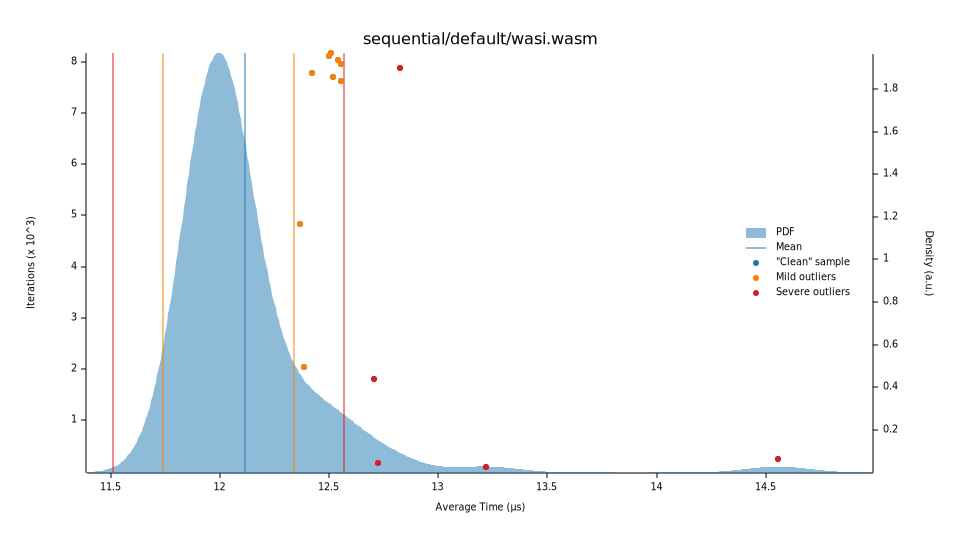
\includegraphics[width=1\linewidth]{images/benches/sequential_default_wasi.pdf}
    \caption{Instantiation distribution of a WASI module with Wasmtime}
    \label{fig:bench:instantiation:wasi}
\end{figure}

\begin{figure}[htbp]
    \centering
        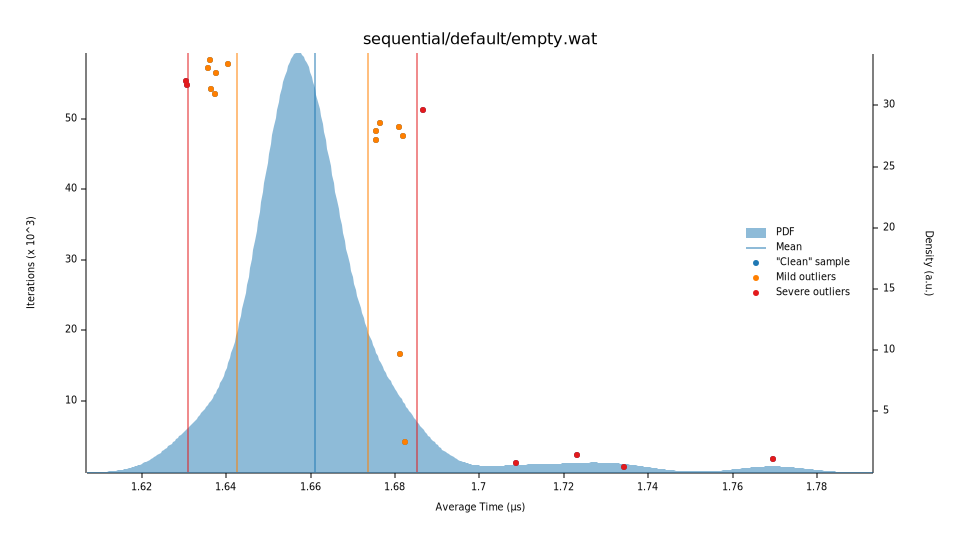
\includegraphics[width=1\linewidth]{images/benches/sequential_default_empty_wasm.pdf}
    \caption{Instantiation distribution of an empty Wasm module with Wasmtime}
    \label{fig:bench:instantiation:empty-wasm}
\end{figure}

\subsection{Programming Languages}
\label{subsec:programming-languages}

\section{Discussion}
\label{sec:discussion}

\begin{figure}[htbp]
    \centering
        \includegraphics[width=1\linewidth]{images/evaluation/curl_performance_metrics.drawio.pdf}
    \caption{Curl performance metrics visualization, redrawn from \cite{speedtestdemon_2021_cheat}}
    \label{fig:eval:curl-metrics}
\end{figure}